

\begin{parag}{Plane}
    For one dimension we had a line, for two dimension we then have... a \important{plane}!!

	\begin{framedremark}
	Remember to put the screen of the plane here
	\end{framedremark}
	We can define our plane as:
	\begin{align*} y = w^{\left(0\right)} + w^{\left(1\right)}x^{\left(1\right)} + w^{\left(2\right)}x^{\left(2\right)} = w^{T}\begin{pmatrix} 1 \\ x^{\left(1\right)} \\ x^{\left(2\right)} \end{pmatrix}  \end{align*}
	All the thing we said to a one dimension fitting is translated into two dimension: Given $N$ noisy plan $\left\{\left(x_i, y_i\right)\right\}$, where $x_i \in \mathbb{R}^2$, find the plane that best fit these observations. Of course as you could have guess, this can be generalized to higher dimensions.
	\begin{itemize}
		\item In dimension $D$, we can write
			\begin{align*} 
				y = w^{\left(0\right)} + w^{\left(1\right)}x^{\left(1\right)} + w^{\left(2\right)}x^{\left(2\right)} + \cdots + w^{\left(D\right)}x^{\left(D\right)} =  w^{T}\begin{pmatrix} 1 \\ x^{\left(1\right)} \\ x^{\left(2\right)} \\ \vdots \\ x^{\left(D\right)} \end{pmatrix} 
			\end{align*}
	\end{itemize}
	Ultimately, whatever the dimension, we can write
	\begin{align*} y = w^{T}x \end{align*}
	With $x \in \mathbb{R}^{D + 1}$, where the extra dimension contains a 1 to account for $w^{\left(0\right)}$.
	
\end{parag}




\begin{parag}{Multi-input linear regression: Training}
    Because the output reamins to one dimension, we can use the same least-square loss function as before, and write training as:
	\begin{align*} \min_w \frac{1}{N}\sum_{i=  1}^{N}d^2\left(\hat{y}_i, y_i\right) \iff \min_w \frac{1}{N}\sum_{i = 1}^{N}\left(x_i^{T}w - y_i\right)^2 \end{align*}
	\begin{subparag}{Note}
	    This has the same form as in the one dimension input case
	\end{subparag}
	Solving this minimization problem involves computing its derivatives w.r.t. the model parameters ($w$) (by using the gradient descent).
\end{parag}

\section{Derivatives and Gradients}
\begin{definition}
The derivative of a function $R\left(w\right)$ of a single variable $w$ is the rate at which $R$ changes as $w$ changes
\end{definition}
\begin{framedremark}
Be careful at this definition, if you have done cs-328 you'll know that derivative as in machine learning and many other topics, use auto-differentiation which is really "different" as how analysis defined derivative. (the 2023 exam asked to derive the load instruction...)
\end{framedremark}
The derivative can also be measured for an infinitesimal change in $w$, startingfrom a point $\overline{w}$, we can write it as:
\begin{align*} R'\left(\overline{w}\right) = \frac{dR}{dw} =  \lim_{\Delta w  \to 0} \frac{R\left(\overline{w} + \Delta w\right) - R\left(\overline{w}\right)}{\Delta w} \end{align*}
\begin{parag}{Minimizing a function}
    In machine learning, we often seek to minimize a function (i.e., the loss function). To minimize such a function, we seek a point where the derivative vanishes, i.e., we search for $w^{\ast}$ such that 
	\begin{align*} \frac{d R\left(w^{\ast}\right)}{dw} = 0 \end{align*}
	For some simple, convex functions, $w^{\ast}$ can be obtained algebraically by solving the corresponding equation
	\begin{subparag}{Remark}
	    This is referred to as closed-form solution
	\end{subparag}
\end{parag}
	\begin{framedremark}

	As former analysis students, we see functions as nice curves that we can draw on a graph which can be specified using usual mathematical language (for instance $f\left(x\right) =  \sin x$). In context of machine learning and auto-diff, this is not always true. Being able to algebraically solve an equation is something 'rare'.
	\end{framedremark}

	\begin{parag}{$ $}
	    For more complicated non-convex functions, there are typically multiple, local minima
	\end{parag}
	



	\begin{parag}{Dealing with multivariate functions}
	    This is nice for one dimension but even our simple case of a model with one dimension had already two parameters ($w^{\left(0\right)}, w^{\left(1\right)}$). In practice, we typically have more than one parameter. To handle this, we rely on the function \important{gradient}. The gradient is a multi-variable generalization of the derivative.\\
		\begin{itemize}
			\item For a function with $D$ parameters, the gradient is a $D$-dimensional vector
			\item Each element of this vector is the partial derivative of the function w.r.t. a single variable, i.e. the derivative of the function w.r.t. one variable while keeping the other constant
		\end{itemize}
		\begin{definition}{Gradient}
		The gradient of a function $R\left(w\right)$ with $w \in \mathbb{R}^{d}$ is denoted by
		\begin{align*} 
			\nabla_w R\left(w\right) = \begin{pmatrix} \frac{\partial R}{\partial w^{\left(1\right)}}  \\ \frac{\partial R}{\partial w^{\left(2\right)}}  \\ \vdots \\ \frac{\partial \mathbb{R}}{\partial w^{\left(D\right)}}  \end{pmatrix} 
		\end{align*}
		Where $\frac{\partial R}{\partial w^{\left(j\right)}} $ denotes the partial derivative w.r.t. variable $w^{\left(j\right)}$.
		\end{definition}
		
	\end{parag}
	



	\begin{parag}{Properties of gradient}
	    \begin{itemize}
			\item The gradient at a point $w$ has the direction of greatest increase of the function $w$ or in other word points to the \important{steepest} 'slope' of the function at the point $v$
	    \end{itemize}
		You can see with this property why the gradient may be useful when looking for minima of a function. If the gradient give us the steepest slope of the function at a given point, when going down this slope, this means that we are going \important{down} the fastest way possible.
	    \begin{subparag}{Little remark for the future}
	        This is nice, going down the slope will make our loss function decrease. But what if it converges onlty to a local minima and not a global one? Doing a gradient descent at a local minima won't work or at least a 'vanilla' gradient descent. A solution to this would be gradient descent with momentum which i don't know if we will see later.
	    \end{subparag}
	\end{parag}
		\begin{figure}[h!]
		\centering
		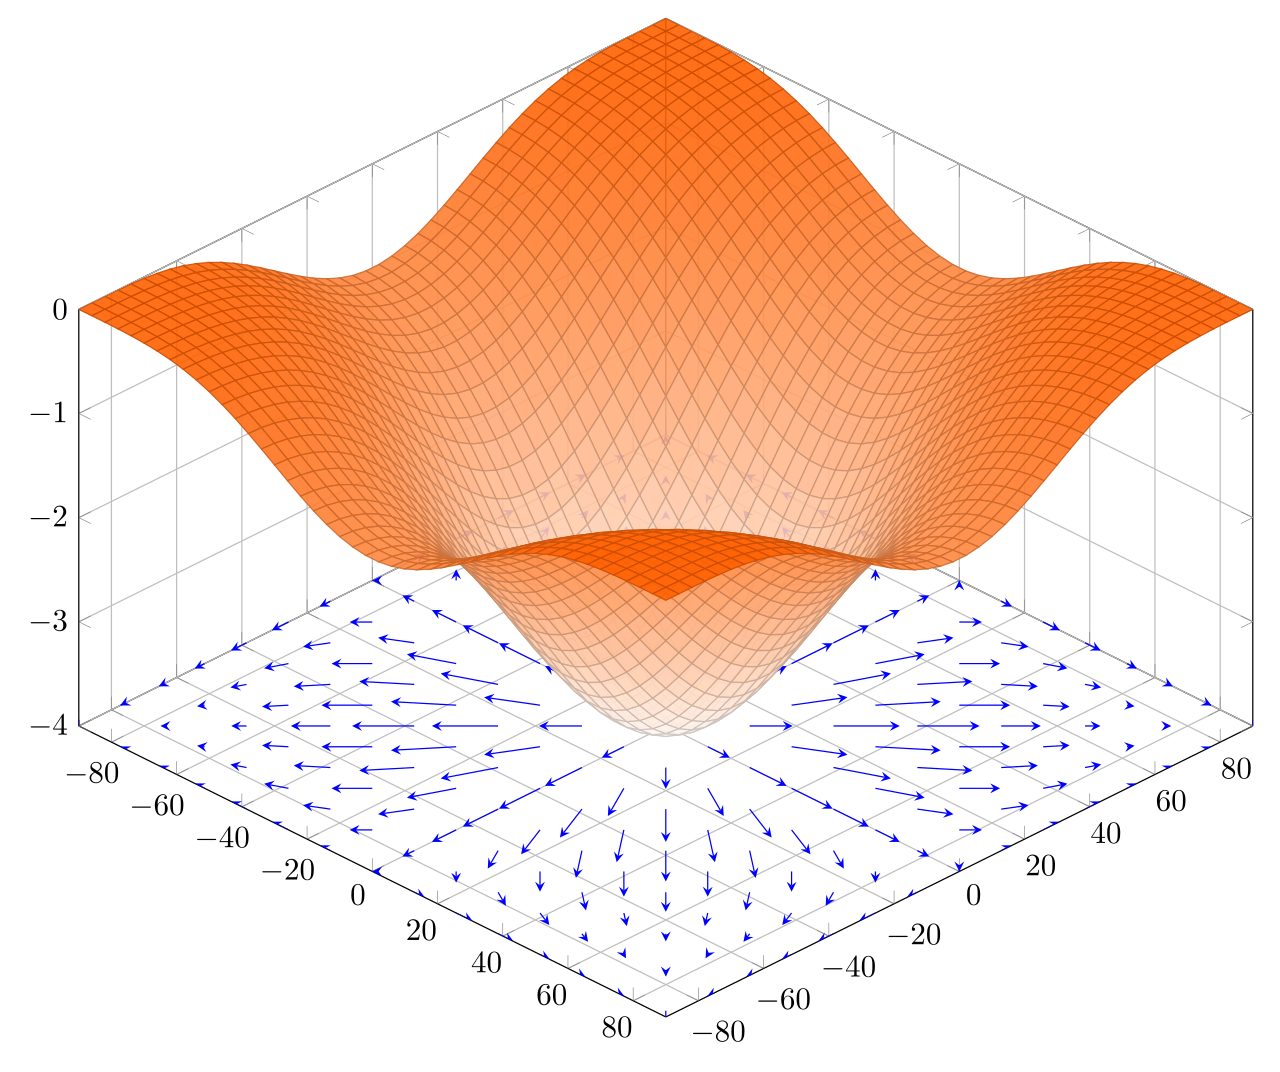
\includegraphics[scale=0.15]{screenshots/2026-02-24_1.png}
		\caption{The gradient of the function $f(x,y) = −(\cos^2x + \cos^2y)^2$ depicted as a projected vector field on the bottom plane. (\href{https://en.wikipedia.org/wiki/Gradient}{wiki})}
		\end{figure}
	\begin{parag}{Linear regression: Solution}
	    If we retake the least-square loss function we defined previously
		\begin{align*} 
			R\left(w\right) = \frac{1}{N} \sum_{i= 1}^{N}\left(w_i^Tw - y_i\right)^2
		\end{align*}
		This is a convex function of $w$, what this means is that the gradient is $0$ only at the global minima. We therefore search a parameter $w^{\ast}$ such that
		\begin{align*} \nabla_w R\left(w^{\ast}\right) = 0\end{align*}
	\end{parag}

	
	\begin{parag}{Gradient Computation}
		Before solving our equation, let us first compute our equation $\nabla_w R\left(w\right)$. Remember first that $R\left(w\right)$ is an average over the $N$ training samples. This means for us that we have $N$ times the same equation for each $i$, which makes the gradient failry easy to compute, we only have to compute:
		\begin{align*} 
			\nabla_w \left(x_i^Tw - y_i\right)^2
		\end{align*}
		By using the chain rule, the function $\left(x_i^Tw - y_i\right)^2$ has the form $f\left(g\left(w\right)\right)$, with $f\left(g\right) =  g^2$. We can compute its gradient as $\frac{df\left(g\right)}{dg} \nabla_wg\left(w\right)$.\\
		$ $\\
		The last trick that we need is the following:
		\begin{theoreme}
		Given two vectors $a, b \in \mathbb{R}^{D}$
		\begin{align*} 
			\nabla_b\left(a^Tb\right) =  a
		\end{align*}
		\end{theoreme}
		\begin{subparag}{Proof}
		    First, recall what the dot product is:
			\begin{align*} 
				a^{T}b =  \sum_{i= 1}^{D}a_ib_i
			\end{align*}
			This give us therefor by definition of the gradient:
			\begin{align*} 
				\nabla_b\left(a^{T}b\right) &= \begin{pmatrix} \frac{\partial a_1b_1}{\partial b_1}  \\ \frac{\partial a_2b_2}{\partial b_2}  \\ \vdots \\ \frac{\partial a_Db_D}{\partial b_D}  \end{pmatrix} \\
				&= \begin{pmatrix} a_1 \\ a_2 \\ \vdots \\ a_D \end{pmatrix} = a
			\end{align*}
		\end{subparag}
		\begin{subparag}{Useful link}
		    Useful rules for matrix (or vector) computations, can be found in the Matrix cookbook:
			\begin{center}
				\href{http://www2.imm.dtu.dk/pubdb/edoc/imm3274.pdf}{http://www2.imm.dtu.dk/pubdb/edoc/imm3274.pdf}
			\end{center}
		\end{subparag}
		Using everything we said before, the gradient of the function $R\left(w\right) =  \frac{1}{N}\sum_{i= 1}^{N}\left(x_i^Tw-y_i\right)^2$ can be computed as:
		\begin{align*} 
			\nabla_w R &= \frac{1}{N}\sum_{i= 1}^{N} \frac{\partial \left(x_i^Tw - y_i\right)^2}{\partial \left(x_i^Tw - y_i\right)} \cdot \frac{\partial \left(x_i^Tw - y_i\right)}{\partial w} \\
					   &= \frac{2}{N} \sum_{i =  1}^{N}\left(x_i^Tw - y_i\right) \cdot x_i
		\end{align*}

	\end{parag}
	\begin{parag}{Solution}
	    To obtain the solution, we search for a $w^{\ast}$ such that 
		\begin{align*} 
			\nabla_w R\left(w^{\ast}\right) = \frac{2}{N} \sum_{i=  1}^{N} x_i \left(x_i^Tw^{\ast} - y_i\right) = 0
		\end{align*}
		\begin{subparag}{Note}
		    The $x_i$ has moved to the front but this make no difference as $\left(x_i^Tw - y_i\right)$ is a scalar
		\end{subparag}
		If we expand here what is inside the sum we have 
		\begin{align*} x_i(x_i^Tw^{\ast}) - x_i \cdot y_i \end{align*}
		If we remove the constant factor $\frac{2}{N}$. Our solution has the following equation
		\begin{align*} 
			\left(\sum_{i= 1}^{N}x_i x_i^T\right)w^{\ast} =  \sum_{i= 1}^{N}x_i y_i
		\end{align*}
		Okay, first let us look a bit more into the dimension of our equation. First $x_i \cdot x_i^T$ gives us a $\left(D + 1\right) \times \left(D + 1\right)$ matrix. $w^{\ast}$ is a $\left(D + 1\right) \times 1$ vector and $\sum_{i = 1}^{N} x_i y_i$ is a $\left(D + 1\right) \times 1$ vector.
		\begin{align*} 
			\underbrace{\left(\sum_{i= 1}^{N}x_i x_i^T\right)}_{\left(D + 1\right) \times \left(D + 1\right)}\underbrace{w^{\ast}}_{\left(D + 1\right) \times 1} =  \underbrace{\sum_{i= 1}^{N}x_i y_i}_{\left(D + 1\right) \times 1}
		\end{align*}

	\end{parag}
	\begin{parag}{Matrix form}
	    As said before, we prefer to use matrix when dealing with machine learning in general, you can also see here that we are doing a sum over product which kind of look like a matrix multiplication. Let us now group all $\left\{x_i\right\}$ and all $\left\{y_i\right\}$ in a matrix and a vector:
		\begin{align*} 
			x = \begin{pmatrix} x_1^{T} \\ x_2^{T} \\ \vdots \\ x_N^{T} \end{pmatrix} = \begin{pmatrix} 1 & x_1^{\left(1\right)} & x_1^{\left(2\right)} & \cdots & x_1^{\left(D\right)} \\  1& x_2^{\left(1\right)} &x_2^{\left(2\right)}  & \cdots  &  x_2^{\left(D\right)}\\ \vdots  & \vdots  &  \vdots & \ddots  & \vdots  \\ 1 & x_N^{\left(1\right)} &  x_N^{\left(2\right)}& \cdots & x_N^{\left(D\right)}  \end{pmatrix} \in \mathbb{R}^{N \times \left(D + 1\right)}
		\end{align*}
		\begin{align*} 
			y =  \begin{pmatrix} y_1 \\ y_2 \\ \vdots \\ y_N \end{pmatrix} \in \mathbb{R}^{N}
		\end{align*}
		With this new notation, we can re-write the solution as:
		\begin{align*} 
			X^{T}Xw^{\ast} = X^{T}y
		\end{align*}
		Sounds familiar to you? this is the definition of the least-square solution we have seen in linear algebra.
		\begin{subparag}{kind of proof?}
		    A nice thing I want to put here which is not part of the course is how do we come up to the relation $X^{T}Xw^{\ast} =  X^Ty$. What we are trying to do (from the beginning of this section), is to minimize the relation $\left\|Xw^{\ast} - b\right\|^2$. By definition of the scalar procut we have the following:
			\begin{align*} 
				\left\|Xw^{\ast} - y\right\|^2 &=  <Xw^{\ast} - y, Xw^{\ast} - y>\\
											   &= <Xw^{\ast}, Xw^{\ast}> - <X^{\ast}, y> - <y, Xw^{\ast}> + <y, y>\\
											   &= w^{\ast T}X^{T}Xw^{\ast} - 2y^{T}Xw^{\ast} + \left\|y\right\|^2
			\end{align*}
			As we want to minimize, we will take its derivative, which make the $\left\|y\right\|^2$ goes away:
			\begin{align*} 
				\frac{\partial }{\partial x} w^{\ast T}X^{T}Xw^{\ast} - 2y^{T}Xw^{\ast} + \left\|y\right\|^2 = 2X^{T}Xw^{\ast} - 2X^{T}y
			\end{align*}
			As we are looking to minimize we seek it to be equal to $0$ which gives us:
			\begin{align*} 
				X^{T}Xw^{\ast} =  X^{T}y
			\end{align*}
		\end{subparag}
		The \important{solution} of this system is given as:
		\begin{align*} 
			w^{\ast} = \left(X^TX\right)^{-1}X^{T}y = X^{\dagger}y
		\end{align*}
		Where $X^{\dagger}$ is known as the \href{https://en.wikipedia.org/wiki/Moore\%E2\%80\%93Penrose_inverse}{Moore-Penrose pseudo-inverse} of $X$ (or directly the pseudo-inverse)
		\begin{subparag}{kind of proof II?}
		    So if I understood correctly what the wiki says, the pseudo-inverse $A^{\dagger}$ and $A^{+}$ is essentially the same. The definition of the pseudo-inverse of a matrix $A$ $A^{+}$ satisfy all of the four criterias, known as the Moore-Penrose condition:
			\begin{align*} 
				A A^{+}A = A\\
				A^{+}A A^{+} = A^{+}\\
				\left(A A^{+}\right)^{\ast} =  A A^{+}\\
				\left(A^{+}A\right)^{\ast} =  A^{+}A
			\end{align*}
			I won't explain what the two lasts means (because I don't know), but why $X^{\dagger} = \left(X^{T}\right)^{-1}X^{T}$?
			Let us define $B$ such that:
			\begin{align*} B =  \left(X^{T}X\right)^{-1}X^{T} \end{align*}
			If we multiply by $X$:
			\begin{align*} 
				XB = X\left(X^{T}X\right)^{-1}X^{T}
			\end{align*}
			And by $X$ again but on the other side
			\begin{align*} 
				XBX = X\left(X^{T}X\right)^{-1}x^{T}X
			\end{align*}
			Which simplify to:
			\begin{align*} 
				XBX = X
			\end{align*}
			For the second criteria, retake our $B$ and multiply by $X$:
			\begin{align*} 
				BX &= \left(X^{T}X\right)^{-1}X^{X}X\\
				   &= I
			\end{align*}
			This directly implies that:
			\begin{align*} 
				\underbrace{BX}_{I}B =  B
			\end{align*}
			And if we had proven the two last criteria we could have concluded that $B = \left(X^{T}X\right)^{-1}X^{T} = X^{\dagger}$.
		\end{subparag}
	\end{parag}
	
	
	\begin{parag}{Test time}
	    As mentioned before, once we have the optimal parameters $w^{\ast}$, we can predict $\hat{y}_t$ for any new value $x_t$. This predicted value is given by:
		\begin{align*} 
			\hat{y}_t = \begin{pmatrix} 1 \\ x_t \end{pmatrix}^{T} w^{\ast} = \left(w^{\ast}\right)^{T}\begin{pmatrix} 1 \\ x_t \end{pmatrix} 
		\end{align*}
	\end{parag}
	\begin{parag}{Evaluation metrics for regression}
	    We can predict but is our prediction good? To be able to measure this we need two things:
		\begin{itemize}
			\item Test data
			\item An evaluation metrics
		\end{itemize}
		We have already spoke about the test data, seperate from the training data, doesn't change the parameters of the model... On the other hand, we have never seen any evaluation metrics before, a value that could tell us wether or not our model is performing well out there in the real world.\\
		$ $\\
		We have defined a loss function before, why not use it as the evaluation metrics? This function is $0$ if the model matches perfectly with all data points, the greater the loss function the greater the offset to the correct value our model is predicting.
	\end{parag}
	\begin{parag}{Mean Squared Error (MSE)}
		\begin{definition}{Mean Squared Error}
	    \begin{align*} \text{MSE} = \frac{1}{N_t} \sum_{i = 1}^{N_t}\left(\hat{y}_i - y_i\right)^2 \end{align*}
		Where $\hat{y}_i$ is the prediction for the test sample $i$ and $y_i$ is the corresponding ground-truth value.
	    \end{definition}
		We can also use the Square-root of the MSE.
	\end{parag}
	\begin{parag}{Mean Absolute Error (MAE)}
		\begin{definition}{Mean Absolute Error}
	    \begin{align*} 
			\text{MAE} =  \frac{1}{N_t}\sum_{i = i}^{N_t}\left\|\hat{y}_i - y_i\right\|
		\end{align*}
	    \end{definition}
		Maybe it can be more intuitive to look at the error as a pourcentage:
		\begin{definition}{Mean Absolute Percentage Error}
		
		\begin{align*} 
			\text{MAPE} = \frac{1}{N_t}\sum_{i= 1}^{N_t}\left\|\frac{\hat{y}_i - y_i}{y_i}\right\|
		\end{align*}
		\end{definition}
	\end{parag}
	
	
	
	
	\subsection{Interpreting a Linear Model}
	First an important thing to check we testing our model is comparin the error value of on the training data \important{and} for the test data. If those two are close this means that our model effectively can generalize to other data. If for instance our model as a very low error on the training data and a high error for the test data, usually this means that the model is \important{overfitting}.
	\begin{center}
	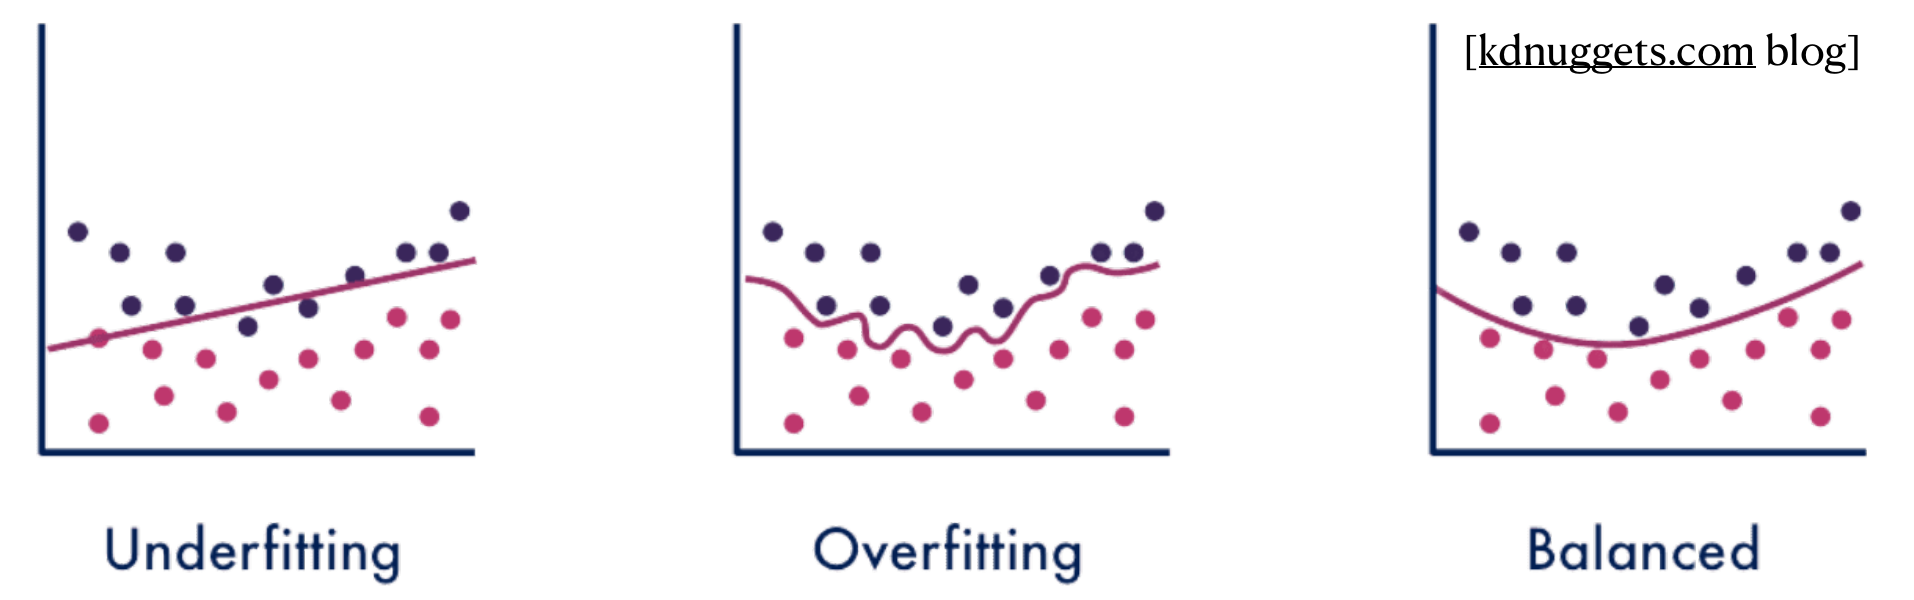
\includegraphics[scale=0.17]{screenshots/2026-02-21.png}
	\end{center}
	The other intresting thing with a linear model is that each value of the model $w^{\left(i\right)}$ directly maps to an attribute of the input. If we take the example of the UCI Wine Quality dataset with the following data:
	\begin{table}[h!]
\centering
\resizebox{\textwidth}{!}{%
\begin{tabular}{|c|c|c|c|c|c|c|c|c|c|c|c|}
\hline
fixed acidity & volatile acidity & citric acid & residual sugar & chlorides & free sulfur dioxide & total sulfur dioxide & density & pH & sulphates & alcohol & quality \\
\hline
7.4 & 0.70 & 0.00 & 1.9 & 0.076 & 11.0 & 34.0 & 0.9978 & 3.51 & 0.56 & 9.4 & 5 \\
7.8 & 0.88 & 0.00 & 2.6 & 0.098 & 25.0 & 67.0 & 0.9968 & 3.20 & 0.68 & 9.8 & 5 \\
7.8 & 0.76 & 0.04 & 2.3 & 0.092 & 15.0 & 54.0 & 0.9970 & 3.26 & 0.65 & 9.8 & 5 \\
11.2 & 0.28 & 0.56 & 1.9 & 0.075 & 17.0 & 60.0 & 0.9980 & 3.16 & 0.58 & 9.8 & 6 \\
7.4 & 0.70 & 0.00 & 1.9 & 0.076 & 11.0 & 34.0 & 0.9978 & 3.51 & 0.56 & 9.4 & 5 \\
\hline
\end{tabular}
}
\caption{Wine quality dataset sample}
\end{table}
After having trained our model we have as the final RMSE:
\begin{itemize}
	\item 0.65 for training data
	\item 0.63 for test data
\end{itemize}
Which is good for us, this means as said before that our model can generalize to other wine. Now let us see what is the parameters of our model:


	\begin{table}[h!]
\centering
\begin{tabular}{|c|c|}
\hline
 & Coefficient \\
\hline
\hline
	fixed acidity & 0.017737 \\
\hline
	volatile acidity & -0.992560 \\
\hline
	citric acid & -0.139629 \\
\hline
	chlorides & -1.590943 \\
\hline
	free sulfur dioxide & 0.005597 \\
\hline
	total sulfur dioxide & -0.003520 \\
\hline
	density & 0.768590 \\
\hline
	pH & -0.4374144 \\
\hline
	sulphates & 0.812888 \\
\hline
	alcohol & 0.301484 \\
\hline
\end{tabular}
\caption{Wine quality parameters}
\end{table}
Having a coefficient close to 0 means that this input is completly 'irrelevant' for our ouput (it is independant as in the probability sense).
\begin{framedremark}
Warning: the magnitude of a coefficient will depend on the magnitude of the corresponding feature/attribute:
\begin{itemize}
	\item A coefficient might be very small imply to compensate for the fact that the range of the feature is very large
	\item This can be addressed by normalizing the data
\end{itemize}

\end{framedremark}

	
\subsection{Linear model with multiple outputs}

Until now we have assumed that the ouput was a single value, i.e., $y_i \in \mathbb{R}$. But in practice, one may want to output multiple values for a given input, i.e., $y_i \in \mathbb{R}^{C}$ with $C > 1$
\begin{parag}{Model}
    To ouput multiple values, the linear model connot just relyu on a vector $w$, because the product $w^{T}x_i$ yields a single value. So let us a matrix $W \in \mathbb{R}^{\left(D + 1\right) \times C}$ such that:
	\begin{align*} 
		\hat{y}_i = W^{T}x_t = \begin{pmatrix} w_{\left(1\right)}^{T} \\ w_{\left(2\right)}^{T} \\ \vdots \\ w_{\left(C\right)}^{T}  \end{pmatrix} 
	\end{align*}
	Since the ouputs are multi-dimensional, we need to slightly modify the loss function, the multi-dimensional counterpart of the $1$D least-square loss is the squared Euclidean distance. Therefore, we can write multi-ouput linear regression as:
	\begin{align*} 
		\min_W \sum_{i= 1}^{N}||W^{T}x_i - y_i||^2
	\end{align*}
\end{parag}
\begin{parag}{Multi-ouput linear regression: Gradient}
    We have our loss function but computing its gradient seems a bit more sophisticated as how we did in the single-ouput linear regression. To compute its gradient, we make use of the following two properties:
	\begin{itemize}
		\item Norm and derivative:
			\begin{align*} ||a||^2 =  a^{T}a \end{align*}
			And thus:
			\begin{align*} \nabla_a ||a||^2 = 2a \end{align*}
		\item Matrix derivative:
			\begin{align*} 
				\nabla_B\left(a^{T}B\right) = a
			\end{align*}
	\end{itemize}
	Thuse, using the chain rule (and replacing $\left(W^{T}x_i - y_i\right)$) with $\left(X_i^{T}W - y_i^{T}\right)$, we obtain the gradient:
	\begin{align*} 
		\nabla_W R = 2 \sum_{i= 1}^{N}x_i\left(x_i^{T}W - y_i^{T}\right)
	\end{align*}
	Setting it to zero means that:
	\begin{align*} 
		\underbrace{\left(\sum_{i= 1}^{N}x_ix_i^{T}\right)}_{\left(D+1\right) \times \left(D + 1\right)}\underbrace{W^{\ast}}_{\left(D + 1\right) \times C} = \underbrace{\sum_{i= 1}^{N}x_iy_i^{T}}_{\left(D + 1\right) \times C}
	\end{align*}
	For the 'training' part, we can again group in a matrix $X \in \mathbb{R}^{ N \times \left( D + 1\right)}$, but the ouputs now need to be grouped in a matrix (and not a vector) as 
	\begin{align*} 
		Y = \begin{pmatrix} y_1^{T} \\ y_2^{T} \\ \vdots \\ y_N^{T} \end{pmatrix}  = \begin{pmatrix} y_1^{\left(1\right)} & y_1^{\left(2\right)} & \cdots & y_1^{\left(C\right)} \\ y_2^{\left(1\right)} & y_2^{\left(2\right)} & \cdots & y_2^{\left(C\right)} \\ \vdots & \vdots & \ddots & \vdots \\ y_N^{\left(1\right)} & y_N^{\left(2\right)} & \cdots & y_N^{\left(C\right)} \end{pmatrix} 
	\end{align*}
	Then, following the same strategy as before, we have:
	\begin{align*} 
		W^{\ast} = \left(X^{T}X\right)^{-1}X^{T}Y =  X^{\dagger}Y
	\end{align*}
\end{parag}


\subsection{Linear Classification}
The goal for now will the same as before however this time instead of having to output a continuous vector, the output will be a class (which is represented by an integer).

\begin{parag}{Binary Classification}
    The easiest classification model we can make is a binary classification one. The output of our model is either 0 or 1.\\
	If we take the following data sets:
	\begin{center}
	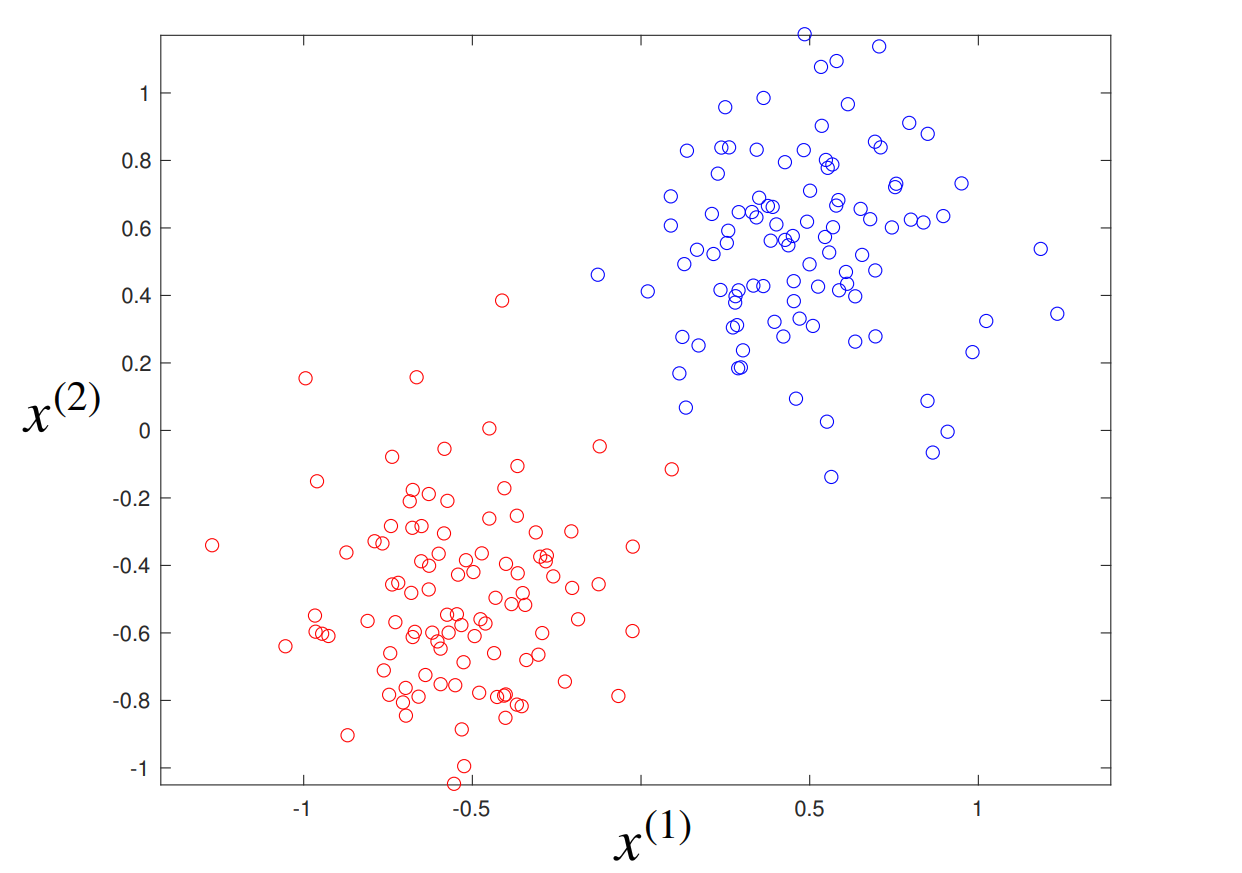
\includegraphics[scale=0.2]{screenshots/2026-02-24.png}
	\end{center}
	\begin{itemize}
		\item We have 2 dimensions input
		\item The label $y \in \left\{-1, 1\right\}$, or $y \in \left\{0, 1\right\}$, is the 1D output
		\item The sample with label 1 are called \important{positive} samples
		\item The sample with label -1 (or 0) are called \important{negative} samples
	\end{itemize}
	But if I have this data in a 2D space, I can also map it to a 3D space by adding the y label into our space. The label acts as the output dimension, just as in a regression problem:
	\begin{center}
	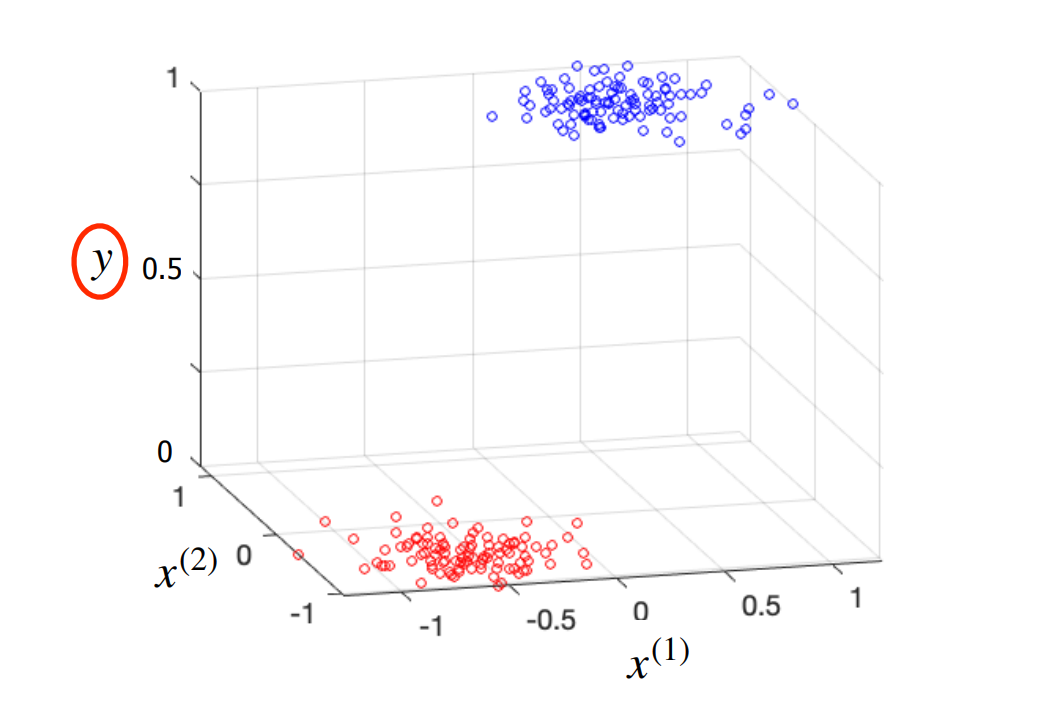
\includegraphics[scale=0.3]{screenshots/2026-02-24_2.png}
	\end{center}
	This means that we can now look at this problem as a regression task, one can tackle classification as a regression task! 
\end{parag}
\begin{parag}{Example (from Andrew Ng's course)}
    The goal is to classify a tumor as benign vs malignant, here's the data:

	But we can still create a model on this data, a linear model which can predict the label as:
	\begin{align*} 
		\hat{y} = w^{\left(0\right)} + w^{\left(1\right)}x
	\end{align*}
	If $\hat{y}$ is small there is a high probability of being and vis versa.\\
	$ $\\
	$ $\\
	To fit the linear model to the training data, the same strategy as for the linear regression can be used:\\
	$ $\\
	Given $N$ pairs $\left\{\left(x_i, y_i\right)\right\}$, we can use the least-square loss to write:
	\begin{align*} 
		\min_W \sum_{i= 1}^{N}\left(x_i^{T}W - y_i\right)^2
	\end{align*}
	Because it has exactly the same formulation as before, the solution is exactly the same, i.e.
	\begin{align*} 
		w^{\ast} = \left(X^{T}X\right)^{-1}X^{T}y
	\end{align*}
	Because we still need to ouput a \important{label}, we will transform our continuous value by using a threshold, for instance:
	\begin{align*} 
		\text{label} = \begin{cases}
			1 \text{ if } \hat{y}_t \geq 0.5\\
			0 \text{ otherwise}
		\end{cases}
	\end{align*}
	Where $\hat{y}_t =  x_t^Tw^{\ast}$. \\
	\begin{subparag}{Remark}
		A general rule when using least-square binary classification is that: the boundary between our two class is of dimension $D$. when we had data of dimension $1$ the decision boundary was a point (i.e. 0.5 above). If our data are in two dimensions, the boundary will be a line.
	\end{subparag}

\end{parag}



